\begin{htmlonly}
\documentclass{article}
\usepackage{makeidx,html}
\usepackage[T1]{fontenc}
\usepackage[dvips]{graphicx}
\usepackage{francais}
\input ex31.ptr
\end{htmlonly}
\startdocument
\index{section!figure}

Cette section montre comment inclure une figure 
PostScript\cite{bib-PS} dans un document \LaTeX. 
La \hyperref{figure}{figure }{}{Fpsfig} 
est ins�r�e dans le texte � l'aide de la commande 
\verb!
\includegraphics{colorcir}!.
\index{figure}
\index{PostScript}
\begin{figure}[h]
\htmlimage{thumbnail=0.4}
\centering
  \begin{tabular}{c@{\qquad}c}
    
\includegraphics[width=3cm]{colorcir} &
    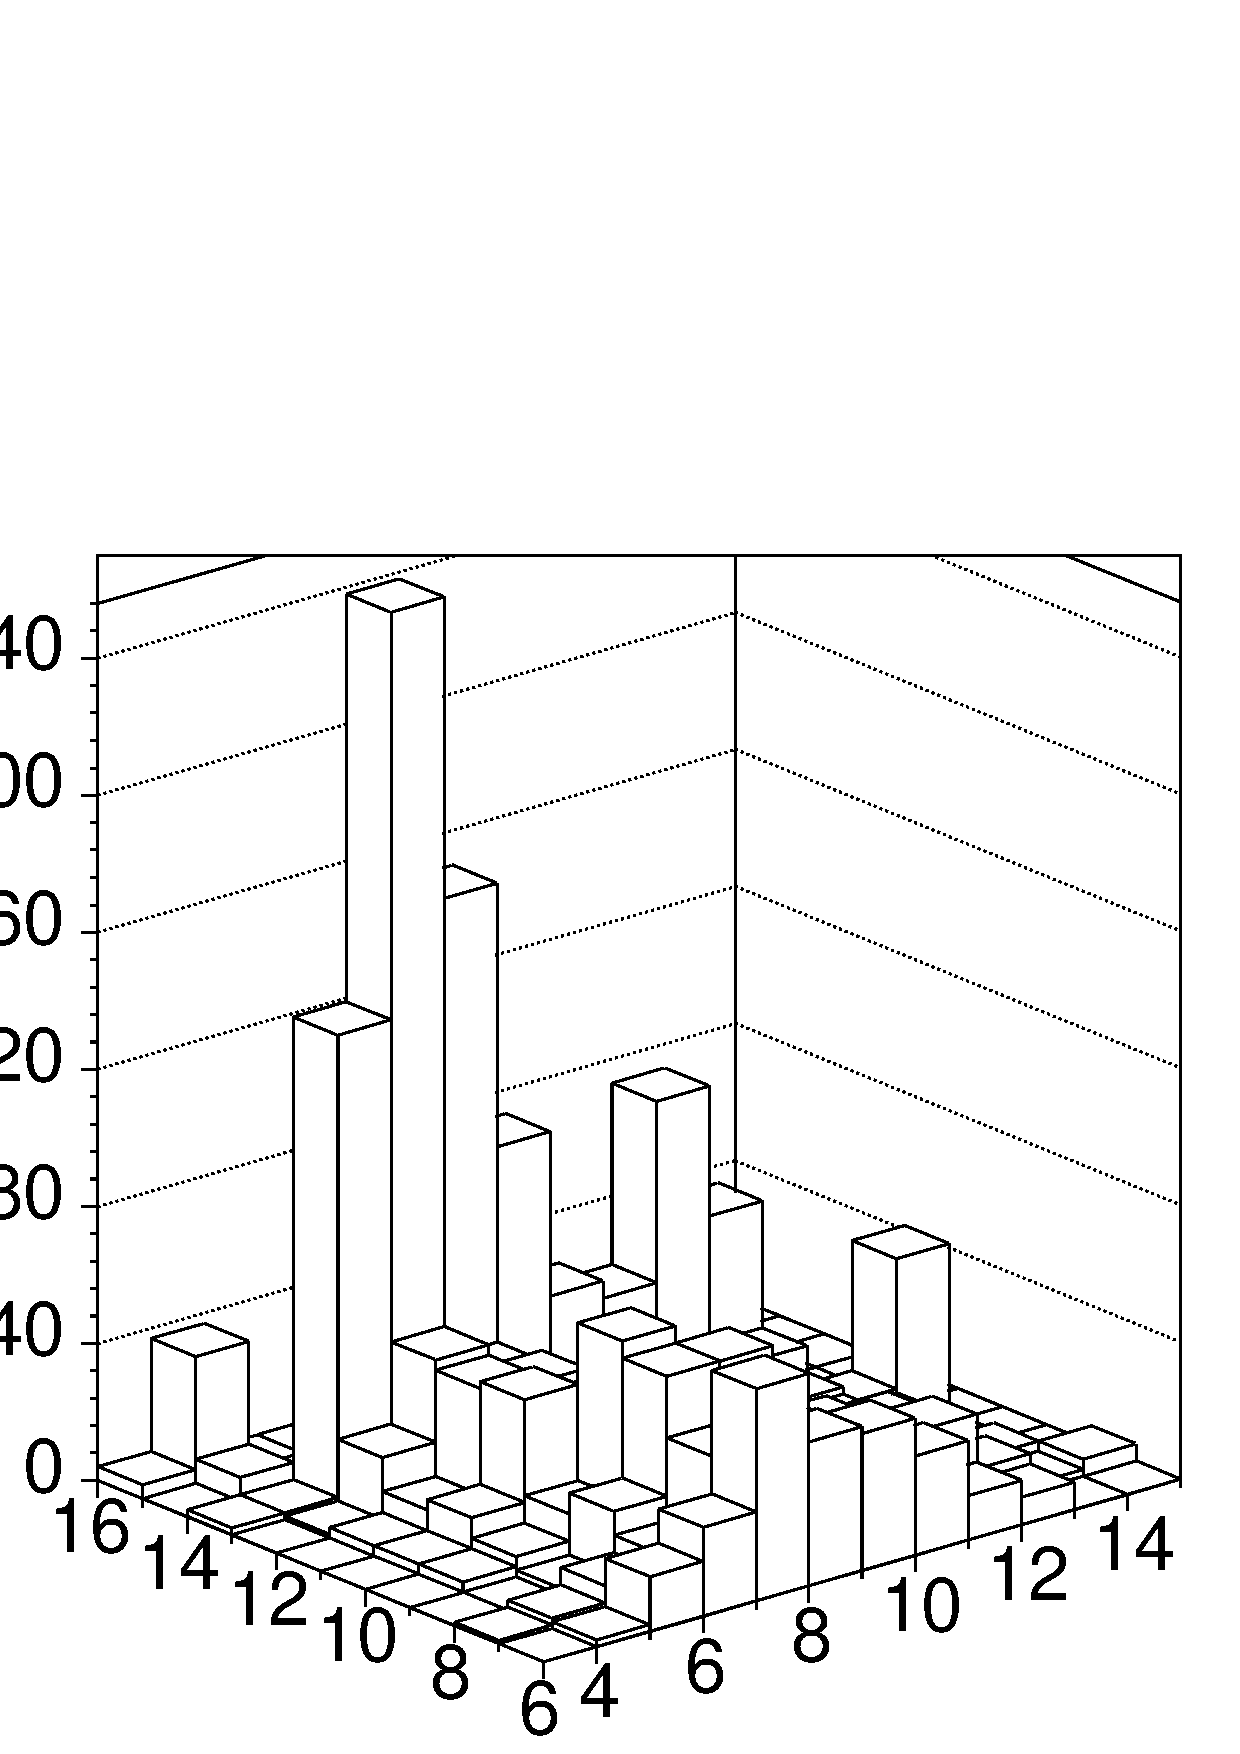
\includegraphics[width=3cm]{tac2dim} 
  \end{tabular}
  \caption{Deux images EPS}\label{Fpsfig}
\end{figure}
